\chapter{Rectifier}
\section{Theory and related work} \label{sec:literature_rectifier}
A basic half-wave rectifier consists of a diode in series with a sinusoidal input voltage. This allows only the positive cycle of the input to appear at the output. Adding a shunt/filter capacitor to the rectifier's output allows for current to flow continuously as the capacitor discharges during the cutoff period of the diode \cite{Neamen:Microelectronics}.


\section{Design} \label{sec:design_rectifier}

\textbf{\textit{Design rationale}} \\
For this design, the main consideration is that the capacitor is large enough to supply current to the rest of the circuit at the required voltage. This is calculated in Equation \ref{eq:rectifier_capacitor}. However, the current flowing through the diode is also a concern as a \SI{0.5}{\ampere} fuse is installed in the design. So, it must be ensured that any transient charging currents are not large or sustained enough that the fuse blows. The 1N4007 diode used here has a peak reverse voltage of \SI{700}{\volt}\cite{1N4007} which is more than sufficient.


\noindent\textbf{\textit{Design calculations}} \\
\textit{Capacitor calculation:}
\begin{equation}\label{eq:rectifier_capacitor}
\begin{split}
        dQ &= i \times dt = C(V_{pk} - V_{min}) \\ 
        C &= \frac{\SI{200}{\milli\ampere} \times 0.02}{\SI{18}{\sqrt{2}}-0.7-12} = \SI{313.6}{\mu\farad}
\end{split}
\end{equation}
Ideally, a $\SI{330}{\mu\farad}$ capacitor would be used. However, due to the voltage rating of the available capacitors, two $\SI{220}{\mu\farad}$ capacitors were instead used.

\textit{Diode current\cite{Neamen:Microelectronics}:}
\begin{equation}
\begin{split}
    i_{D,peak} &= i_{load}(1 + \pi\sqrt{\frac{2V_M}{V_r}})
    = \SI{200}{\milli\ampere} \times (1 + \pi\sqrt{\frac{2(18\sqrt{2}-0.7)}{18\sqrt{2}-0.7-12}}) \\
    &= \SI{1.438}{\ampere}
\end{split}
\end{equation}

This is higher than the fuse rating. However, the melting time of the fuse at this current is: $ \frac{0.215}{1.438^2} = \SI{104}{\milli s}$\cite{Fuse}. This is much higher than the maximum positive cycle period of 10ms. Hence, it can be assumed to be safe enough.


\noindent\textbf{\textit{Circuit diagram}}
\begin{figure}[h]
    \centering
    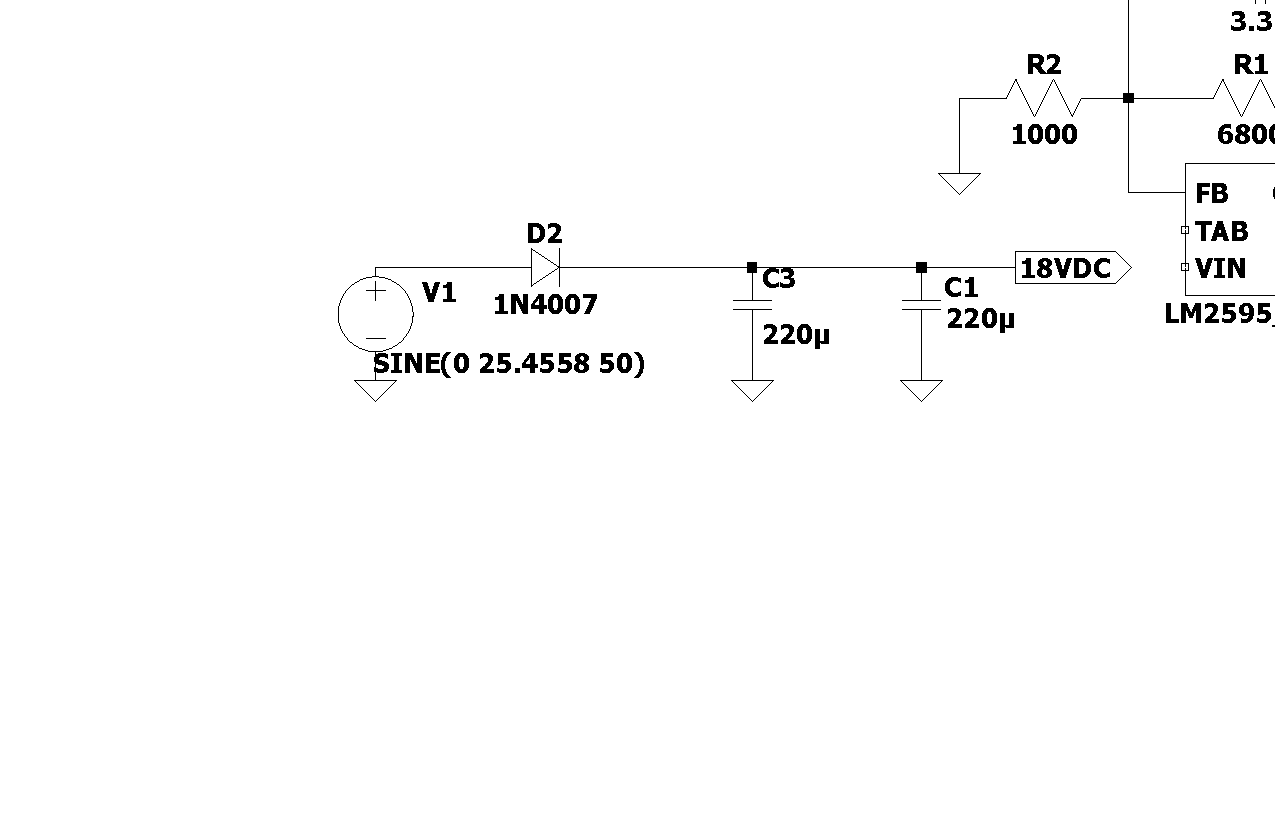
\includegraphics[clip, trim = 3cm 7cm 2cm 3.7cm,width = 0.75\linewidth]{Figures/rectifier_circuit.pdf}
    \caption{Half wave rectifier circuit}
    \label{fig:rectifier_circuit}
\end{figure}


\section{Simulation} \label{sec:simulation_rectifier}

\begin{figure}[h] 
 \centering
 
    \begin{subfigure}[]{0.5\linewidth}
        \centering
        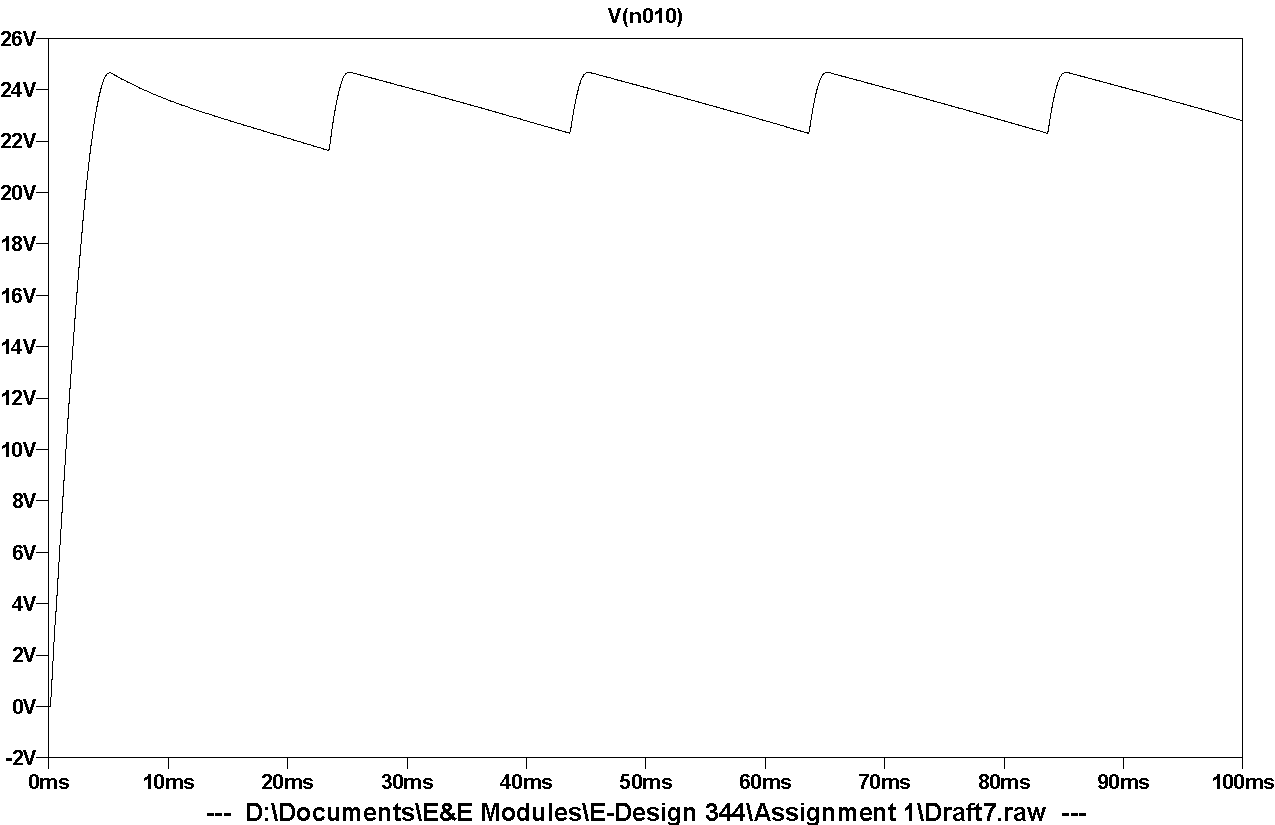
\includegraphics[width=1.\linewidth]{./Figures/rectifier_simulate.pdf}
        \caption{Simulated rectifier output.}
        \label{fig:rectifier_simulation}
    \end{subfigure}
    \begin{subfigure}[]{0.44\linewidth}
        \centering
        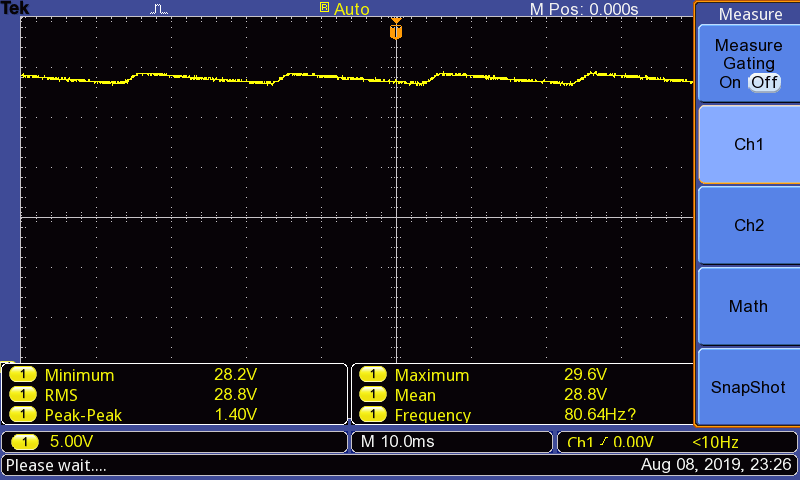
\includegraphics[width=1.\linewidth,clip,trim = 0.3cm 0cm 2.5cm 0cm]{./Figures/rectifier_test}
        \caption{Measured rectifier output.} 
	    \label{fig:rectifier_measurement}
    \end{subfigure}
    
\caption{Rectifier simulated and measured output}
\end{figure}

\section{Measurements} \label{sec:measurements_rectifier}



